\chapter{Background}

% Background to explain context and significance of the question we are addressing.

% genotype and phenotype
% PCG heavily tied to games. Sometimes used to describe ``creating game content automatically''. It doesn't need to be about games though.
% Spelunk and Occupancy Regulated Extension (OCE): https://www.researchgate.net/publication/221157490_Procedural_level_generation_using_occupancy-regulated_extension
% Unexplored and Cyclic Dungeon Generation (article source https://ctrl500.com/tech/handcrafted-feel-dungeon-generation-unexplored-explores-cyclic-dungeon-generation/)(park source https://www.youtube.com/watch?v=mA6PacEZX9M)

% PCG in Games
% Minecraft and Minecraft Dungeons
% Terraria / Starbound
% Dead Cells
% Dwarf Fortress
% Enter the Gungeon
% The Binding of Isaac
% Spelunky
% Unexplored
% Borderlands Series
% Diablo
% Spore
% Civilization Series
% No Man's Sky

% PCG is not just about games! Harder to find about movies though...
% Originted from games as well (hardware limits etc).
% \cite{massive} was used for LOTR and James Cameron's Avatar though

% Needed to avoid having it in glossary
% voxels (minecraft), low poly (Superhot VR), cel shading (wind waker)
% https://www.flickr.com/photos/playstationblogeurope/35145507761

% Related works
% CityGen
% Introversion
% Papers

% What is PCG? (definition and explain with examples)
PCG is a family of algorithms that automatically and randomly generates synthetic media such as 3D models, textures, items, quests, levels and music~\cite[p.1]{pcg_in_games}.
Typically, this generation is achieved by combining manually designed assets with stochastic, yet controllable algorithms.
The algorithms are restricted by manually designed rules to only produce quality content, and utilize randomness within these constraints to generate diverse results~\cite{gamasutra}.
For instance, a correct PCG algorithm for car generation would always produce functional cars, but the resulting cars will still vary by configurable properties such as wheels, seats, size, engine, price, and name.

% History and significance
% In the early 1980s, PCG was primarily used in games as a workaround for the limited storage space~\cite[p.4]{pcg_in_games}.
% In recent years, however, the technique has gained a lot of attraction in modern games for generating compelling and replayable experiences.
% Games such as Diablo~\cite{diablo} features procedural generation for the creation of the maps and as well as the placement and number of items and monsters~\cite[p.4]{pcg_in_games}.
% In Spore~\cite{spore}~, the animation of the creature the player designs use procedural animation techniques\cite[p.4]{pcg_in_games}.
% Furthermore, the popular game Minecraft~\cite{minecraft} makes use of PCG techniques extensively for generating everything from the cave-systems to the mountains to the whole world~\cite[p.4]{pcg_in_games}.
% Procedural generation can be used to generate pretty much any virtual content you could imagine.
% Evident from the use of PCG in big commercial games there is a demand from the game industry to create large, impressive and unique environments for their player base to explore.

% \begin{figure}[h!]
%  \centering

%  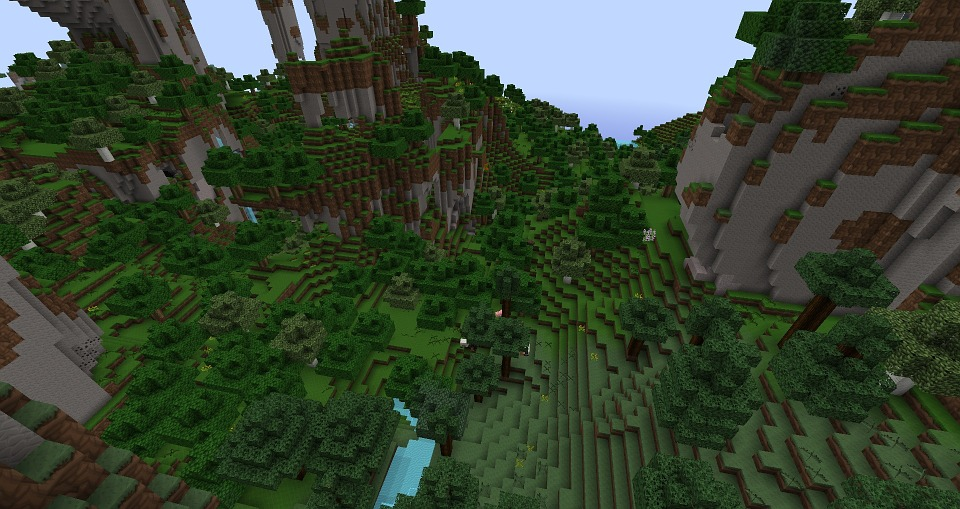
\includegraphics[width=0.8\textwidth]{figure/minecraft.jpg}
%  \caption{Example of voxels in Minecraft. \cite{minecraft_img}}

%  \label{fig:minecraft}
% \end{figure}